\documentclass[10pt]{article}

\usepackage[margin=1in]{geometry}
\usepackage{amsmath,amsthm,amssymb}
\usepackage{graphicx}
\usepackage{subfig}
\usepackage{float}
\usepackage{wrapfig}
\usepackage{multicol}
 \usepackage{booktabs}
 \usepackage{hyperref}
 \hypersetup{
 	colorlinks=true,
 	linkcolor=blue,
 	filecolor=magenta,      
 	urlcolor=cyan,
 }

\graphicspath{ {/Users/clay/Documents/research/TGE-SP21/assignments/images/} }

\begin{document}

% --------------------------------------------------------------
%                         Start here
% --------------------------------------------------------------

\title{Assignment 3}%replace X with the appropriate number
\author{Geosc 597-003\\
Techniques of Geophysical Experimentation} %if necessary, replace with your course title \\

\maketitle


%\noindent{\large \textbf{Due: 03 March}}


\section*{Activity Wheatstone Bridge Construction and Analysis}

We’re going to build a calibrated load cell (force measurement device) using a rock sample and a Wheatstone bridge.  If you do good work you’ll be able to measure the deformation that you can produce with your hands!  \\

Let’s start by looking at an example.  Notice that this device is powered by a simple 9V battery and that the deformation you produce is readily (easily?) measured. \\


\begin{figure}[ht]
	\centering
	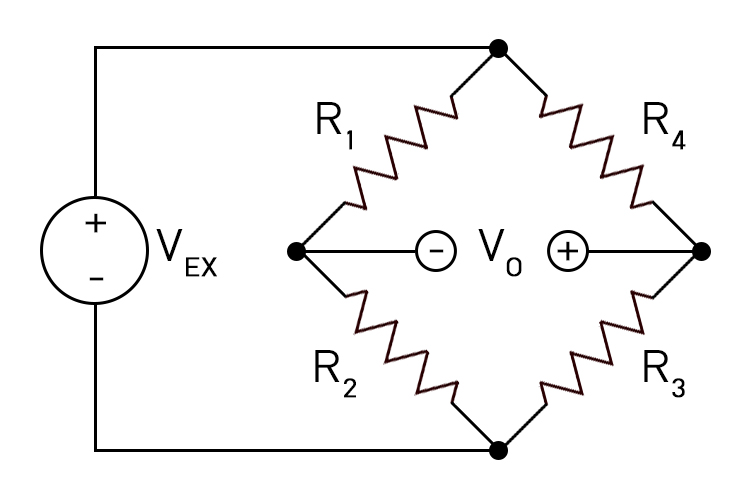
\includegraphics[width=0.3\columnwidth]{wheatstone_bridge}
	\caption{Circuit diagram for Wheatstone Bridge.}
	\label{fig:wheatstone}
\end{figure}
 
$ V_{EX} $ = 9V and we’re measuring the voltage $ V_0 $ with the strip chart recorder and the voltmeter.\\

Notice what happens when you squeeze the surface that contains the gauges. The magnitude and sign of the change in voltage is proportional to strain or shortening.  \\

How much shortening do you think you’re producing? Guess: \line(1,0){30} (m) \line(1,0){10} \\

Ok, let’s estimate/calculate the shortening.  We can start by assuming that you can produce a force of 10 N.  For the 5x5cm surface, 10 N would produce 4 kPa. Actually, the stress will be higher because we should use the area of your finger. So, let’s guess that you’re producing 100 kPa, which is what you’d get from 10 N on 1cm$ ^2 $ area.  A stress of 100 kPa on a granite block with $ E $=50 GPa should produce a strain of 2e-6, which amounts to 0.1 µm on our 5 cm block. Hmmm, impressive eh? \\

Let’s call the surface with the gauges the top surface.  What do you think will happen if you squeeze the bottom surface? The top surface should expand, right?  Before you try it, what do you think will happen to the magnitude and sign of the voltage change. Will it be the same sign and approximately the same magnitude as the shortening that you produced by squeezing the top? \\

Guess (circle one) sign is the same/opposite? magnitude is smaller/larger?\\

What did you observe \line(1,0){30} ? Make a sketch of what happens. \\

\begin{figure}[ht]
	\centering
	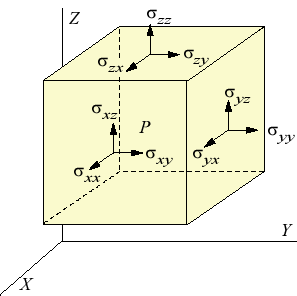
\includegraphics[width=0.3\columnwidth]{stresses.png}
	\caption{Stress state on unit cube.}
	\label{fig:stresses}
\end{figure}

Now let’s look a bit more carefully at the electrical circuit and how this works. We can use this sketch to think about what happens when you squeeze the sample. Let’s imagine that the gauges are on the z plane (plane perpendicular to z) and that the force of squeezing is in the x direction on the x plane. \\

If the force is applied in the x direction we have a stress $ \tau_{xx} $ and a strain $ \epsilon_{xx} = \tau_{xx}/E $ where $ E $ is Young’s modulus.   Because the material’s volume remains essentially constant, a shortening in the $ x $ direction means that the material expands slightly in the $ y $ and $ z $ directions. This is the Poisson effect.  The Poisson expansion is a strain ($ \epsilon_{zz} $ and $ \epsilon_{yy} $) of opposite sign to $ \epsilon_{xx} $.  The ratio of the lateral to axial strain is defined as the Poisson’s ratio, $ \nu_{zx} = -\frac{\eta_{zz}}{\epsilon_{xx}}$.  This is an elastic material property.  For an anisotropic material it’s possible that  $ \nu_{zx} \neq \nu_{yz}$ but our granite is essentially isotropic, so we’ll assume that this is true.
\\

Ok, so now let’s connect this sketch to our Wheatstone bridge.  Note that the bridge is set up so that gauges R1 and R3 are parallel and that they are perpendicular to R2 and R4.  So when R1 and R3 are shortened R2 and R4 expand.
Make a sketch of the block with the gauges and of the wheatstone bridge. 
\vspace{4cm}


What do you suppose happens when you shorten a strain gauge?  Right, the length of the wire decreases.  The wire is actually quite long but it’s laid out in a compact form, back and forth, see Figure \ref{fig:str_gauge}. Do you see how this is actually quite a long wire, even though the length of the strain gauge is small?  
\begin{figure}[ht]
	\centering
	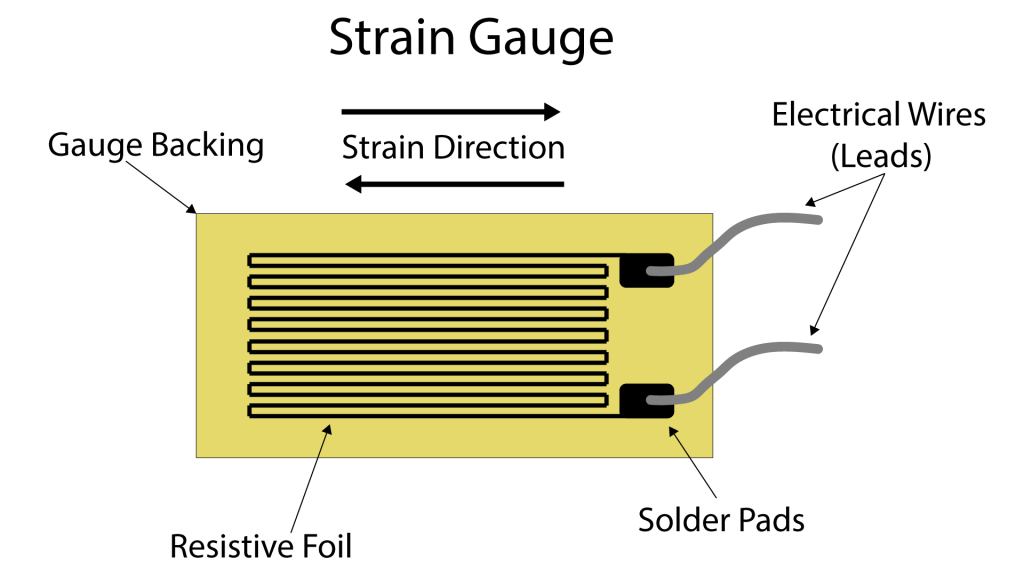
\includegraphics[width=0.3\columnwidth]{strain_gauge.png}
	\caption{Strain gauge components.}
	\label{fig:str_gauge}
\end{figure}

The resistance R of a wire (measured in Ohms) is given by:  $ R = \frac{\rho L}{A} $ where $ \rho $ is the material resistivity of the wire, L is the length of the wire, and A is the cross-sectional area of the wire.  If the length of the wire increases by $ \Delta L $, its resistance will change by $ \Delta R $, and we can write:
\\

$ R + \Delta R = \frac{\rho (L + \Delta L)}{A} $  (assuming the change in A is negligible).\\

Then if we divide both sides by $ R $, we have: \\

$ \frac{R}{R} + \frac{\Delta R}{R} = \frac{\rho L}{A R} + \frac{\rho \Delta L}{A R}$\\

Recall from above that $ R = \frac{\rho L}{A} $. Thus $ \frac{\rho L}{A R} = 1$, which reduces to \\

$ \frac{\Delta R}{R} = \frac{\rho \Delta L}{A R} = \frac{\Delta L}{L} = \epsilon $ \\

So, the proportional change in $ R $ is equal to the strain of the wire. That’s a first order result which makes strain gauges extremely useful.
There’s one catch and it’s called the Gauge Factor. Due to non-ideal behavior of the strain gauge, we need to use a proportionality constant called the Gauge Factor ($ GF $) to correct for the fact that the change in resistance for a given strain is larger than the above equation predicts.
\\
$ \epsilon = \frac{\Delta R}{R} \frac{1}{GF} $\\

The GF is typically about 2.0\\

So, let’s look at a few things with the example block.  
\begin{enumerate}
	\item Measure the resistance of the strain gauges.  You’ll want to unplug the battery and look carefully at how the wires are connected.  Use a volt ohm meter to clarify any uncertainty you have about the wiring set up.  For example, you can verify how wires are connected in the bridge by making sure you have zero resistance between each end of the wire.  What is the resistance of each gauge in the bridge ?  Please write a sentence explaining how you got this number?
	\item Measure the voltage of the battery. It should be 9V. What is it?
	\item Now imagine that we load the rock with a stress $ \tau_{xx} $ (see diagram above) of 100 kN.  Assuming a $ GF $ of 2, what should be the resistance change, $ \Delta R $ of each gauge? 
	\item For a resistance change of $ \Delta R $, what should the voltage be at Vo in the diagram on page 1?
	\item Use a weight to load the rock sample. Measure the weight and predict the values of $ \Delta R $ and $ V_0 $. Then measure the values. How does your calculation compare to your measurement? 
	\item You will be given some strain gauges, a piece of rock and some wire. Make your own wheatstone bridge and test it, as above. In the coming weeks we’ll load your sample in the Biax and measure it’s properties.
\end{enumerate}



%\noindent\textbf{\textit{Do the following:}}
%\begin{enumerate}
%		\item Build an Arduino Voltmeter using the LCD screen -- as Clay demonstrated in class \#3.
%		\item Set up the wiring for a blinking LED and use your 10k potentiometer (SIK) to control the blinking rate. 
%		\begin{enumerate}
%			\item Measure the voltage with your Arduino Voltmeter and convert the output that you measure from the pot. (sensorValue) to voltage.
%			\item Write the voltage to the serial monitor at the same rate that your LED is blinking.
%			\item What happens when you vary the position of the pot?
%		\end{enumerate} 
%		\item Produce a fully commented code and write a brief summary of what you’ve done.
%\end{enumerate}
%
%\begin{table}[h!]
%	\footnotesize
%	\centering
%	\begin{tabular}{@{}ll@{}}
%		\multicolumn{2}{c}{\textbf{Grading Rubric}} \\ \midrule 
%		\multicolumn{1}{l}{\textit{Problem}}   & \textit{Points}   \\ \midrule 
%		\#1                    & 25       \\ \midrule
%		\#2            & 15       \\ \midrule
%		\#3            & 10       \\ \midrule
%		Total                            & 50       \\ \bottomrule
%	\end{tabular}
%\end{table}
%
% \clearpage
% 
% 
% 
%\section*{Activity 2 - Temperature and Humidity Sensor}
%
%Build a temperature and relative humidity sensor using the DHT11 chip supplied with your kit.  Study the technical docs (link below) and try to do your wiring and write your code from scratch, without using any on-line resources.  In the end, if you need help, go ahead and look online and/or see one of us if you need help. \url{https://github.com/clay-wood/TGE-SP21/tree/main/resources/Elegoo_starter_kit/Datasheet}\\
%
%\noindent Document your setup with a wiring diagram or photos (captioned), and concise description as necessary. It should be easy for others to replicate what you've done. 
%
%
%\begin{table}[h!]
%	\footnotesize
%	\centering
%	\begin{tabular}{@{}ll@{}}
%		\multicolumn{2}{c}{\textbf{Grading Rubric}} \\ \midrule 
%		\multicolumn{1}{l}{\textit{Topic}}   & \textit{Points}   \\ \midrule 
%		Functioning Sensor                   & 10       \\ \midrule
%		Original Code            & 5       \\ \midrule
%		Documentation            & 10       \\ \midrule
%		Total                            & 25       \\ \bottomrule
%	\end{tabular}
%\end{table}
%
%
%\section*{What to upload to Canvas}
%You should upload the following with \textit{consistent file names}:
%
%\begin{itemize}
%	\item Your Arduino codes. Make sure it works before you upload.
%	\begin{itemize}
%		\item \textbf{Fully comment your code!} 
%		\item \textbf{Naming convention:} username\_projectX.ino\\
%		Example: cew52\_blinky2.ino, cew52\_stoplight.ino.
%		\item Put all Arduino codes for this assignment in a project folder. 
%	\end{itemize}
%
%	\item Relevant movies or photos.
%	\begin{itemize}
%		\item \textbf{Naming convention:} username\_LED\_bright.mov
%	\end{itemize}
%	\item Summary from Activity 1 and your concise project documentation from Activity 2.
%	\item Put all files inside of a directory named: username\_assignment3
%\end{itemize}

%\vspace{2cm}



\end{document}